% Header {{{
% vim: ft=tex:fdm=marker
\documentclass[a4paper]{article}

% Plugins {{{
    \usepackage[T1]{fontenc}
    \usepackage[utf8]{inputenc}
    \usepackage[icelandic]{babel}

    \usepackage{url}
    % Graphics
        \usepackage{graphicx}
        \graphicspath{
            {visualisation/graphics/}
        }
% }}}

\title{Krónan eða Evran fyrir Ísland?}
\author{Árni Dagur}
% }}}
\begin{document}
\maketitle

\section{Inngangur}

Lengi vel hefur innganga Íslands inn í Evrusvæðið verið umræðumál hér á landi, og magnaðist sú umræða mjög eftir hrunið mikla árið 2008. Hægt er að móta rök með og á móti upptöku hennar, og er hægt að finna fræðimenn sem tala fyrir hendi beggja hliða. Í þessu riti verður farið yfir þessi rök og í lok þess lýsir höfundur sinni persónulegri skoðun.

Í viðtali við \textit{The Guardian} lýsti háttsettur Íslenskur embættismaður sem ekki vildi láta nafns síns getið vantrausti sínu til krónunnar. \textit{''The Krona is dead. We need a new currency. The only serious option is the euro.''} sagði hann.\cite{traynor_2009}

\section{Rök með}

\subsection{Aukinn stöðugleiki gjaldmiðils}
\begin{figure} %{{{Volatility.png
    \centerline{
        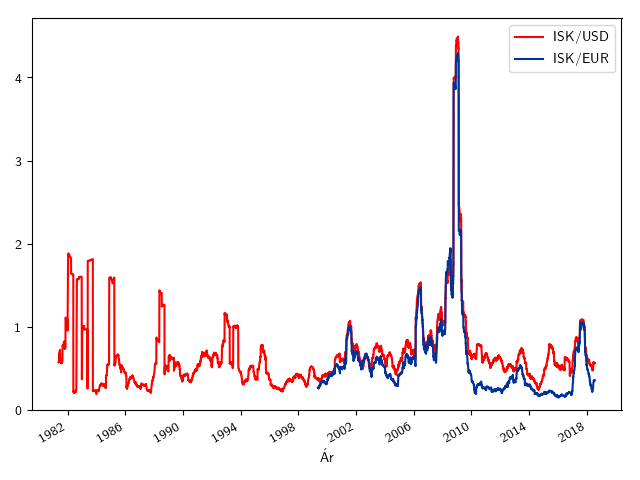
\includegraphics{volatility.png}
    }
    \caption{Staðalfrávik prósentubreytingar með 90 daga rúllandi ramma. Gögn koma frá Seðlabanka Íslands.}
    \label{fig:volatility}
\end{figure} %}}}

Árið 2008 var stöðugleiki krónunnar miðað við önnur lönd rannsakaður af René Kallestrup, hagfræðing Seðlabanka Íslands. Niðurstaða þessarar rannsóknar leyddi í ljós að óstöðugleiki íslensku Krónunnar er í \textit{''the high end among developed market currencies, and the average is now slightly above countries like New Zealand and Australia. However, the average volatility remains substantially below that of high-yielding emerging market currencies.''} Stöðugleiki Evrunnar er aftur á móti þó nokkuð meiri – svipaður Bandaríkjadalnum.\cite{icb_volatility_2008}

Á Mynd \ref{fig:volatility} sést óstöðugleiki Krónunnar miðað við Bandaríkjadalinn og Evruna vel. Hann er skilgreindur sem staðalfrávik prósentumuns á 90 daga rúllandi ramma.

\subsection{Minni þörf á að geyma varaforða erlenda gjaldmiðla}

Vegna þess eins að Evrusvæðið hafi verið stofnað hefur þörf Seðlabanka Íslands til þess að geyma erlenda gjaldmiðla minnkað. Í staðinn fyrir marga sjóði fyrir hvert Evrópuríki sem Ísland gerir viðskipti við (þýsk Mörk, franskir Frankar, spænskir Pesóar, etc) getur hann haldið einn Evrusjóð fyrir öll ríki Evrusvæðisins.

Við upptöku Evrunnar gæti Ísland minnkað forða sinn á gjaldmiðlinum enn frekar\cite{saga_evropusamrunans}, en árið 2017 voru Evrur 30\% forðans.\cite{icb_annual_2017}

\subsection{Aukin viðskipti við Evrusvæðið}

Árið 2004 gerði Þórarinn G. Pétursson, sem nú er aðalhagfræðingur Seðlabanka Íslands, rannsókn í samvinnu við breskan hagfræðing þar sem reynt var að leggja tölu á kosti þess að ganga inn í Evrusvæðið. Notast var við svokallað \textit{Gravity Model of Trade} til að leggja mat á áhrif semeigilegs gjaldmiðils, og gjaldmiðlaóstöðuleika á alþjóðleg viðskipti, líkt og lýst var af Rose et al (2000).(?) Þeir komust að þeirri niðurstöðu að það megi búast við 60\% viðskiptaaukningu við það að ganga í Evrusvæðið. Helmingur þess gróða mætti rekja til þess eins að ganga í ESB, en hinn helminginn til upptöku Evrunnar. Ástæðan fyrir því má einmitt að mörgu leyti rekja til ofanlýstra punkta.\cite{icb_wp_26}

Í kennslubókinni \textit{Economics} sem er kennd í þessum áfanga er sú staðreynd að alþjóðaviðskipti gerir báða aðila betur af lýst sem ein af 10 grundvallarreglum hagfræðinnar. Aukning nær 60 prósentustigum á alþjóðaviðskiptum við Evrusvæðið væri því mjög góð fyrir Ísland, sérstaklega þar sem stór hluti alþjóðaviðskipta Íslendinga eru nú þegar við Evrópusambandið (?).

\section{Rök á móti}

\subsection{Missir á eigin peningastefnu}

\subsubsection{Dæmið um Grikkland}

Í venjulegum kringumstæðum þar sem land hefur hefur fullt vald yfir gjaldmiðli sínum mun það bregðast við miklu atvinnuleysi með því að prenta meiri pening. Það lækkar virði gjaldmiðilsins og þar með hækkar ferðamannastraum, fjárfestingar, og gróða útflutningsgreina. Ef atvinnuleysi er lágt, aftur á móti, mun það prenta minni pening og þar með hækka kaupmátt og lækka verð á vörum (Klein, 2015). Þetta getur þó Grikkland ekki gert af því hvernig Evrusvæðið er sett upp. Þó að Grikkland stjórni sínum eigin ríkisfjármálum, stjórnar Seðlabanki Evrópusambandsins  peningastefnu þess (Pogorelec). Styrkur gjaldmiðils sem er tilvalinn fyrir Þýskaland, þar sem atvinnuleysi er 4.2\% (The European Union) er allt annar en styrkur gjaldmiðils sem er tilvalinn fyrir Grikkland, þar sem atvinnuleysi er 23.2\% (The European Union).

\subsubsection{Dæmið um Ísland}

Eftir hrunið mikla árið 2008 var Ísland í sambærilegri stöðu, en þó höfðum við stjórn á okkar peningastefnu. Sú staðreynd reyndist Íslendingum vel: Fall krónunnar leyddi til ófordæms áhuga erlendra ferðamanna á eyjunni sem ódýran áfangastað,\cite{worldfinance_2015} en ferðamennska til landsins er nú 320\% af því sem hún var árið 2006, fyrir hrunið.\cite{hagstofan_passengers} Útflutningsgreinar Íslands, sérstaklega fiskiðnaðurinn, sáu einnig stórar aukningar á tekjum sínum. Ísland er nú alþjóðlegt kennslubókardæmi um hvernig hrun gjaldmiðils getur leitt til hraðrar efnahagsbötnunar.\cite{worldfinance_2015}

Ef Ísland hefði verið með Evruna árin eftir hrunið mikla 2018, værum við því líklega í sömu stöðu og Grikkland.

\subsection{Skortur á sameiginlegri fjármálastefnu}

Eins og Berger et al. lýstu í ritgerð sinni \texit{''Revisiting the Economic Case for Fiscal Union in the Euro Area''} er nokkur hætta falin í því að deila sameiginlegri peningastefnu en ekki fjármálastefnu.\cite{fiscal_union}

\section{Niðurstaða}

Því miður er ég ekki hagfræðingur, og treysti ég mér því ekki til þess að taka þessu stóru ákvörðun um upptöku Evrunnar fyrir hönd Íslendinga. Rök er þó greinilega hægt að færa fyrir báðum hliðum.

\newpage
\bibliography{bibliography}
\bibliographystyle{plain}

\end{document}
